\documentclass{article}
\usepackage[a4paper, portrait, margin=2.5cm]{geometry}
\usepackage{graphicx}
\usepackage{relsize}
\usepackage[utf8]{inputenc}

\usepackage{hyperref}

\usepackage{bm,nicefrac,xfrac}
\usepackage{amsmath}
\newcommand{\mathup}[1]{\text{\textup{#1}}}

\newenvironment{itquotation}
{\begin{quotation}\itshape}
	{\end{quotation}}
\newenvironment{itquote}
{\begin{quote}\itshape}
	{\end{quote}}

\usepackage{siunitx}



\usepackage[
citestyle=authoryear,
backref=true,
]{biblatex}
\bibliography{../references/DP-experiment.bib} % or
%\bibliography{/users/thomas/onedrive/phd/literature/bibliography.bib} % or
% \addbibresource{<database>.<extension>}


\begin{document}

\author{Thomas Wodzinski}
\title{Coherence measurements with double pinholes at FLASH2 \\[0.2em]\smaller{} - collection of notes -}
\maketitle


\section{explanations, terminology, theory}
\begin{enumerate}
	\item on model sources: \cite["radiation from model sources", ch. 5.2.2, pp. 233-]{MandelWolf1995-Opticalcoherencequantum} 
	\item if \cite{GorobtsovMercurioBrennerEtAl2017} were able to calculate a global degree of coherence for FLASH1, why can it not be calculated with these DPH  measurements? They were also assuming a Gaussian-Schell-model.
	\item \cite[p.817, right column]{McNeilThompson2010} The normalized beam emittance cannot be higher than $ \epsilon_n < \gamma \lambda_1 / 4 \pi$ to ensure good spatial/transvere coherence. This was derived by Kim1986... How can I check this for our measurements? How "good" will the coherence be due to "good" emittance?
	\item Saldin2000 pp. 407, ch. 6.3.2 Transverse Coherence
	\item use "Coherence area" instead of "coherence length": "transverse or spatial coherence length" $ \xi $ is not the same as the "(longitudinal?) coherence length" $ L_\mathup{c} $ related to the coherence time $ \tau_\mathup{c} $ ... equations  \begin{itquote}
		In some systems, such as water waves or optics, wave-like states can extend over one or two dimensions. Spatial coherence describes the ability for two points in space, x1 and x2, in the extent of a wave to interfere, when averaged over time. More precisely, the spatial coherence is the cross-correlation between two points in a wave for all times. If a wave has only 1 value of amplitude over an infinite length, it is perfectly spatially coherent. The range of separation between the two points over which there is significant interference defines the diameter of the coherence area, Ac [13] Coherence length, often a feature of a source, is usually an industrial term related to the coherence time of the source, not the coherence area in the medium.) Ac is the relevant type of coherence for the Young's double-slit interferometer. It is also used in optical imaging systems and particularly in various types of astronomy telescopes. Sometimes people also use "spatial coherence" to refer to the visibility when a wave-like state is combined with a spatially shifted copy of itself.
	\end{itquote} (\url{https://en.wikipedia.org/wiki/Coherence_(physics)#Spatial_coherence})
	\item Mutual coherence function looks at both temporal and spatial coherence ... Are we measuring only the spatial coherence? or a "mutual" coherence?
	\item beam emittance:
	\begin{itquote}
		Emittance is a property of a charged particle beam in a particle accelerator. It is a measure for the average spread of particle coordinates in position-and-momentum phase space and has the dimension of length (e.g., meters) or length times angle (meters times radians).
	\end{itquote}
	\url{https://en.wikipedia.org/wiki/Beam_emittance}
	\item "geometrical emittance":
	\item \url{https://conf-slac.stanford.edu/sssepb-2013/sites/conf-slac.stanford.edu.sssepb-2013/files/S3EPB_Lecture1_Huang.pdf}
	\item \url{https://staff.aist.go.jp/arimoto-h/Thesis/node1.html}
	\item first vs second-order correlations?
	\item "shift invariant" coherence: spatial coherence only dependent on the separation of the point, independent on the position inside the beam ...
	\item \cite[p.48, ch. 3.2]{Jaegle2005-CoherentSourcesXUV}: Modes of Free Radiation Field
	summarizes \cite[ch. 4.5 and 5.5]{MandelWolf1995-Opticalcoherencequantum}
	"coherent-mode representation", mutual coherence function $ \Gamma $, cross-spectral density function $ W $, spectral degree of coherence $ \mu $, complex degree of coherence $ \gamma $, global degree of spatial coherence of a one-dimensional Gaussian source model $ q(\nu) $, number of modes increases the smaller the global spatial degree of coherence $ q $ becomes
	\item van Cittert-Zernike theorem: \cite[p.47, 129]{Jaegle2005-CoherentSourcesXUV}
	\item Gaussian-Schell models: \cite[p. 130]{Jaegle2005-CoherentSourcesXUV}
	"both intensity and coherence obey a Gaussian distribution" according to \cite{MandelWolf1995-Opticalcoherencequantum}, which page?
\end{enumerate}

\begin{figure}[h]
	\centering
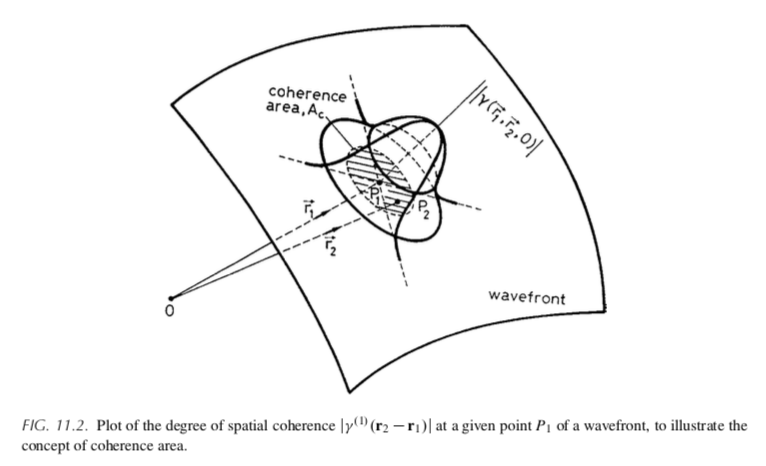
\includegraphics[width=0.7\linewidth]{Svelto2010fig11p2}
	\caption{from \cite{Svelto2010}}
	\label{fig:svelto2010-fig11}
\end{figure}

\begin{figure}[h]
	\centering
	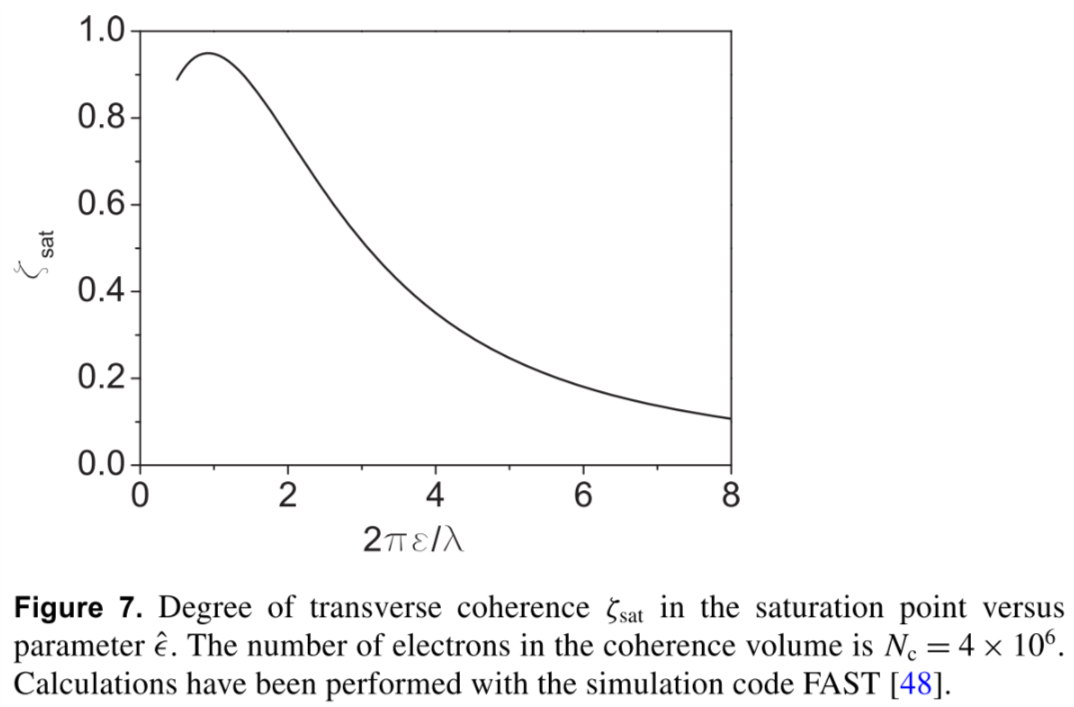
\includegraphics[width=0.7\linewidth]{SaldinSchneidmillerYurkov2010fig7.png}
	\caption{from \cite{SaldinSchneidmillerYurkov2010}}
	\label{fig:saldinschneidmilleryurkov2010fig7}
\end{figure}


\subsection{Schell-model}

\cite[(p. 1, para. 2)]{BurdetShimomuraHiroseEtAl2016} say about the Gaussian-Schell model:

\begin{itquotation}The synchrotron sources can be described as partially coherent sources using various models.\textsuperscript{7} For example, the Gauss-Schell model has been used to model synchrotron radiation,\textsuperscript{8,9} in which the sources are viewed as random superpositions of coherent Gaussian beams.
\end{itquotation}

\begin{itemize}
	\item "Gaussian-Schell" or "Gauss-Schell" is used in literature
	\item "Schell" is a guy, it is not a reference to shells
	\item there exist also "generalized Schell" models
	\item can Gauss-Schell models only be used for synchrotrons, but not for FELs?
\end{itemize}



\cite{BartelsPaulGreenEtAl2002}

\subsection{Blind-deconvolution to recover the partially coherent intensity}

The measured intensity can be expressed as a convolution (see \cite[(eq.33)]{VartanyantsRobinson2001} \cite[(eq.23)]{WilliamsQuineyPeeleEtAl2007} (citing \cite{LinPatersonPeeleEtAl2003} (citing \cite{Nugent1991})), \cite[(eq.1)]{WhiteheadWilliamsQuineyEtAl2009} and \cite[(eq.5)]{ClarkHuangHarderEtAl2012}):

\[I_{\mathup{pc}} = I_\mathup{c} \ast \mathcal{F}(\gamma)\]

where $I_{\mathup{pc}}$ and $I_c$ are the partially coherent intensity and the coherent intensity, respectively, and $\mathcal{F}$ represents the Fourier transformation. $\gamma$ is termed as the normalized spatial coherence function, transverse ($r$) to the direction of the wave field propagation.

The transverse coherence length $\xi_\mathup{T}$ can be measured as the FWHM of the $\mathcal{F}(\gamma)$ at the detector plane. (reference?) 

\[\gamma \propto \exp\!\left[-\frac{r}{2\sigma}\right]\]


\[\left( I_{\mathup{pc}},\mathcal{F}(\gamma)_{\mathup{est}}\right)  \longrightarrow \left( I_\mathup{c}, \mathcal{F}(\gamma)_{\mathup{rec}} \right)  \]


\subsection{transverse coherence length $\xi_\mathup{T}$, global degree of coherence $\zeta$}

\begin{itquotation}
   Within the framework of the Gaussian Schell model (GSM), which is widely used to describe synchrotron radiation from an undulator, the CDC and the intensity distribution of the X-ray beam are assumed to be Gaussian functions. In this case, a global degree of coherence can be introduced, which characterizes the transverse coherence properties of the beam by one number [13,21,22] \cite{SingerSorgenfreiMancusoEtAl2012}

\[
\zeta = \left( \frac{\xi_\mathup{T}}{\sigma_\mathup{B}} \right) \left[ 4 + \left( \frac{\xi_\mathup{T}}{\sigma_\mathup{B}} \right)^2 \right]^{-1/2}
\]

$\xi_\mathup{T}$ is the transverse coherence length defined as the root mean square (rms) width of the CDC and $\sigma_\mathup{B}$ is the rms width of the beam intensity distribution. $\zeta$ varies from zero for incoherent to one for coherent radiation. 
\end{itquotation}
\begin{flushright}
	(from \cite[eq.5]{BagschikFroemterMuellerEtAl2016a})
\end{flushright}

\subsection{terminology}

from \cite{Huang:2013nka} using \cite{Goodman2015-StatisticalOptics2e} and \cite{SingerSorgenfreiMancusoEtAl2012}

\begin{itemize}
	\item coordinate system: $\vec{x} = (x,y,z) $
	\item beam propagates longitudinally along $ z $
	\item transverse coordinates are $ (x,y) $ 
	\item scalar electric field $ E(\vec{x}, t) $
	\item $ t $: arrival time of the signal at a particular $ z $ location
	\item mutual coherence function (MCF):
	\begin{equation}\label{key}
	\Gamma(\vec{x}_1,\vec{x}_2,t_1,t_2) = \left\langle E(\vec{x}_1, t_1), E^*(\vec{x}_2, t_2) \right\rangle_T
	\end{equation} (\cite[eq.?]{Huang:2013nka})
	\item mutual coherence function (MCF): 
	\begin{equation}\label{key}
	\Gamma_{12}(\tau) = \left\langle E^*(\vec{r}_1, t), E(\vec{r}_2, t+\tau) \right\rangle_T
	\end{equation} (\cite[eq.1]{SingerSorgenfreiMancusoEtAl2012} using \cite[eq.(5.2-8),p.175]{Goodman2015-StatisticalOptics2e}, \cite[eq.(4.3-9), p.163]{MandelWolf1995-Opticalcoherencequantum} introduced by \cite[eq.(1-2)]{Wolf1955})
	\item $ ^* $: complex-conjugate
	\item $ \left\langle \right\rangle_T $: ensemble average over many radiation pulses over a time interval $ T $
	\item ensemble average is a time average for stationary and ergodic fields ... see \cite[p.162]{MandelWolf1995-Opticalcoherencequantum}
	\item $ z $ is considered as the independent variable and suppressed in the expressions as much as possible
	\item the complex degree of (mutual) coherence (C.D.C.) is defined as the normalized mutual coherence function (a second-order correlation function in terms of field (\cite[eq.4]{BagschikFroemterMuellerEtAl2016a}))):
	\begin{equation}\label{key}
	\gamma(\vec{x}_1,\vec{x}_2,t_1,t_2) = \frac{\Gamma(\vec{x}_1,\vec{x}_2,t_1,t_2)}{\sqrt{ I(\vec{x}_1,t_1)  I(\vec{x}_2,t_2)}} 
	\end{equation}
	\item "mutual", because we are looking at the coherence coming from the two beams at pinhole $ P_1 $ and $ P_2 $. If we are only looking at temporal coherence of one beam, then one could say complex degree of "self-"coherence (\cite[eq. (5.2-12)]{Goodman2015-StatisticalOptics2e})
	\item $ I(\vec{x},t) = \Gamma(\vec{x},\vec{x},t,t) $ is the radiation intensity
	\item Typical x-ray pulse duration generated from the electron bunch is much longer than the coherence time of undulator radiation and of FELs. This let's us approximate (why?):
	\begin{equation}\label{eq:coherencefunction_approx}
	\gamma(\vec{x}_1,\vec{x}_2,t_1,t_2) = \gamma(\vec{x}_1,\vec{x}_2,t_1-t_2)
	\end{equation}
	\item $ \gamma(\vec{x}_1,\vec{x}_2,0) $ describes transverse/spatial coherence
	\item $ \gamma(0,0,\tau) $ describes longitudinal/temporal coherence
	\item "Transverse coherence or spatial coherence describes the degree to which the phase of the wave is correlated at two distinct points in the transverse plane."
	\item interference pattern in Young's double slit experiment: two slits located at $ \vec{x}_1 $ and $ \vec{x}_2 $ at the plane position $ z = 0 $ will form an interference pattern in the far-field far from the slits.
	Total intensity on the screen:
	\begin{align}
	I_\mathup{tot} &= 
	  \left| \left\langle E(\vec{x}_1, t-t_1)\right\rangle \right|^2 
	+ \left| \left\langle E(\vec{x}_2, t-t_2)\right\rangle \right|^2
	+ 2 \mathup{Re}\left[ \left| \left\langle E(\vec{x}_1, t-t_1) E^*(\vec{x}_2, t-t_2)\right\rangle \right| \right] \\
	&= I(\vec{x}_1) + I(\vec{x}_2) + 2 \sqrt{I(\vec{x}_1) I(\vec{x}_2)} \mathup{Re}\left[ \left| \gamma(\vec{x}_1, \vec{x}_2, t_1-t_2) \right| \right]
	\end{align}
	$ t_1 $ and $ t_2 $ are the times taken by signals from each slit to reach the screen at time $ t $.  Equation \ref{eq:coherencefunction_approx} was used to simplify the last step. At the center of the screen where $ t_1 = t_2 $, the fringe visibility is given by the amplitude of the transverse correlation function $ \gamma(\vec{x}_1, \vec{x}_2, 0) $.
	\item  $ \left| \gamma(\vec{x}_1, \vec{x}_2, 0) \right| $ "amplitude" is equal to "modulus"?
	\item modulus of the CDC = fringe visibility ?
	\item if not in the far field ... modulus of the CDC is what? the "degree of coherence" instead of "complex degree of coherence"?
	\item "total degree of transverse coherence" / "coherence fraction":
	\begin{equation}\label{key}
	\zeta = \frac{\iint \left|  \gamma(\vec{x}_1, \vec{x}_2, 0) \right|^2 I(\vec{x}_1) I(\vec{x}_2) d\vec{x}_1 d\vec{x}_2}
	{\int I(\vec{x}_1) d\vec{x}_1 \int I(\vec{x}_2) d\vec{x}_2}
	\end{equation}
	so, the intensity gets weighted with the modulus of the complex degree of coherence at each position and normalized with the integrated intensity of the beam:
	\begin{equation}\label{key}
	\zeta = \frac{\int \left|  \gamma(x, 0) \right| I(x) dx }
	{\int I(x) dx}
	\end{equation}
	\item $ \nicefrac{1}{\zeta} $ is a measure of transverse mode numbers.
	\item fully transversely coherent: $ \zeta = 1 $ 
	\item \cite[eq. (6)]{SingerSorgenfreiMancusoEtAl2012} defines $ \zeta $ as the \textit{"normalized" degree of coherence} instead of "global" or "total", citing \cite[eq. 11]{SaldinSchneidmillerYurkov2008} and \cite{VartanyantsSingerMancusoEtAl2011}
	\begin{equation}\label{key}
	\zeta = \frac{\iint \left|  \gamma(\vec{x}_1, \vec{x}_2, 0) \right|^2 \left\langle I(\vec{x}_1)\right\rangle \left\langle  I(\vec{x}_2)\right\rangle  d\vec{x}_1 d\vec{x}_2}
	{\left( \int \left\langle I(\vec{x}_1) \right\rangle  d\vec{x}_1 \right)^2 }
	\end{equation}
	\item \cite[eq. 11]{SaldinSchneidmillerYurkov2008} uses the term \textit{"degree of transverse coherence"}
	\item !! \cite[pp. 3-4]{VartanyantsSingerMancusoEtAl2011} use the term \textit{"total degree of transverse coherence"}, assuming a Gaussian Schell model an the pinholes at the focus and the pattern in the far-field ... they are using the same equation like \cite[eq. 5]{BagschikFroemterMuellerEtAl2016a}, so why can't I do it?
	\item \cite[eq. 7]{VartanyantsSinger2010} call $ \zeta $ the \textit{"normalized degree of the transverse coherence"}, citing \cite[eq. 11]{SaldinSchneidmillerYurkov2008}. It is not the "degree of coherence" $ q $ (\cite[eq.34]{VartanyantsSinger2010}) from 
	\item $\xi_\mathup{T}$ is the transverse coherence length defined as the root mean square (rms) width of the CDC (\cite[eq.5]{BagschikFroemterMuellerEtAl2016a})
	
\end{itemize}

\subsection{interference in the intermediate zone}

(from Madoud's notes)

Here, the question highlighted in Bartel’s paper (\cite[p.378, par.1]{BartelsPaulGreenEtAl2002}) is discussed: A beam is focused before the pinholes and the pinholes are sampling the curvature of the phase front (and the local tilt is larger than the divergence due to diffraction (?)).

Without any loss of generality, a 1-D model is studied:

Diffraction of light from a circular aperture can represented in the form of Fresnel-propagation in free-space as (\href{https://en.wikipedia.org/wiki/Fresnel_diffraction#The_Fresnel_diffraction_integral}{see wikipedia})

\begin{equation}\label{eq:fresnel-prop1}
	E\left(x, z_p \right)  \simeq - \frac{i}{\lambda z_p} \exp\!\left[ i \frac{k}{2 z_p} x^2 \right] \int_{D-\nicefrac{w}{2}}^{D+\nicefrac{w}{2}}  E^\prime (x', 0)  \exp\!\left[ i \frac{k}{2 z_p} x'^2 \right]  \exp\!\left[ i \frac{k}{z_p} \vec{x} \cdot \vec{x}'  \right]  \mathop{dx'}
\end{equation}

($ z_p $: ?)

where $ (x,x') $ form the coordinate system, $ E' $ is the wave field illuminating the aperture, $ k $ is the wave vector, $ D $ is the off-center distance in positive $ x' $-direction and $ w $ is the aperture diameter. When the illuminating pulse is planar $ E' $ is a constant number. But, if a focused beam illuminates the pinhole located at $ z_0 $ downstream of the focus, $ E' $  can be expressed ideally as a constant amplitude with a quadratic phase term (why?)

\begin{equation}\label{eq:E_prime}
E^\prime(x^\prime, z_0) = E^\prime_0 \exp\!\left[ i \frac{k}{2 z_0} x'^2 \right]
\end{equation}

Substituting eq. (\ref{eq:E_prime}) in eq. (\ref{eq:fresnel-prop1}) yields:

\begin{equation}\label{eq:fresnel-prop2}
E\left(x, z_p \right)  \simeq - \frac{i}{\lambda z_p} \exp\!\left[ i \frac{k}{2 z_p} x^2 \right] \int_{D-\nicefrac{w}{2}}^{D+\nicefrac{w}{2}}  E^\prime_0 \exp\!\left[ i \frac{k}{2 z_M} x'^2 \right]  \exp\!\left[ i \frac{k}{z_p} \vec{x} \cdot \vec{x}'  \right]  \mathop{dx'}
\end{equation}

where $ z_M = \frac{z_p \cdot z_0}{z_p+z_0} $ is the scaled distance. Eq. \ref{eq:fresnel-prop2} is called the Fresnel scaling theorem and considered as a propagation routine when the light to be propagated is itself spherical (\cite[("Appendix B", pp. 397-400)]{Paganin2006}).

The classical transition from Fresnel to Fraunhofer diffraction is met when the quadratic term of the integrand can be expressed as unity, which in turn requires:

\begin{equation}\label{eq:classicaltransition}
	\frac{k \left( D \pm \frac{w}{2} \right)^2 }{2 z_M} \ll 2 \pi
\end{equation}

When ineq. (\ref*{eq:classicaltransition}) is not satisfied, eq. (\ref{eq:fresnel-prop1}) gradually collapses. Therefore, one can define a cut-off value for $ D $ as:

\begin{equation}\label{eq.cut-off}
	|D| \ll \beta \sqrt{2 \lambda z_M} - \frac{w}{2} = D_\mathup{cut-off}
\end{equation}

In a double-pinhole experiment $ D $ corresponds to the pinhole separation. $ \beta $ is supposed to compensate the geometrical wavelength variations.

In short, relying solely on the Fresnel number, in case of a divergent illumination of the double-pinhole plate, might not be enough assessment for interpreting the intensity observed. Referring to the experimental geometry, $ z_M $ is approximately 0.85 ($ z_p = \SI{6}{m} $ and $ z_0 = \SI{1}{m} $), $ \lambda = \SI{13.5}{nm} $ and $ w = \SI{10}{\micro\meter} $. Thus, $ D_\mathup{cut-off} \approx \SI{20}{\micro\meter} $. It should be noted that $ D $ has been determined for an ideal experiment and it may potentially change with the systematical variations. Considering the wavelength and geometry described in \cite{VartanyantsSingerMancusoEtAl2011} for a Young's double pinhole experiment (with a negligible wavefront curvature) at LCLS, $ D_\mathup{max} $ is found to be $ D_\mathup{max} \approx \SI{60}{\micro\meter} $. As reported, they used a series of pinholes ranging from \SIrange{2}{15}{\micro\meter} which automatically satisfied ineq. (\ref*{eq:classicaltransition}).



\subsection{questions}

Masoud wrote on 29.09.2018:

\noindent\rule{\textwidth}{1pt}
\begin{itquote}
	\begin{enumerate}
		\item What exactly does mean the Global degree of coherence (GDC)? 
		\begin{enumerate}
			\item You're using the general version of Schell theorem as a convolution, not the Gaussian-Schell model (one of the requirements of the Gaussian-Schell model is an app. a constant beam which is satisfied in synchrotrons but not at FELs), so is the GDC a universal quantity applies to all sources? 
			\item Under which condition could you safely use the GDC concept at FELs? 
			\item Which property of FEL sources (specifically FLASH II) may potentially break / or strongly hold the GDC?
		\end{enumerate}
		
		\item I recall eq. 5 in Kai's paper and rename $\nicefrac{\xi_\mathup{T}}{\sigma_\mathup{B}}$ as $A$. Consider the highest extreme of $\zeta$ (GDC) which is $1$, square both side of the eq. 5, we would obtain $4+A^2 = A^2$ (Eq.1).
		Eq.1 is valid when $A$ approaches infinity which in turn requires $ \xi_\mathup{T} \gg \sigma_\mathup{B} $ (Eq.2) 
		\begin{enumerate}
			\item Can you describe a situation in which one would be able to observe Eq.2 in a double-pinhole experiment?
			\item Could you generally explain under which condition/s the spatial coherence length of an electric field is extremely larger than its intensity FWHM?
		\end{enumerate}
	\end{enumerate}
\end{itquote}
\noindent\rule{\textwidth}{1pt}

\begin{itemize}
	\item How is the generalized Schell model used in my case? I am using it for the deconvolution?
\end{itemize}

\subsection{various}

Intensity profile:

\[  I(r)=I_{0} \exp \left(-2{\frac {r^{2}}{w^{2}}}\right)  \]

\[ \sigma = \frac{\mathrm{FWHM}}{\sqrt{2 \ln(2)}} \]

$ \sigma $: root-mean-square (rms) width

beam diameter on wikipedia: \url{https://en.wikipedia.org/wiki/Beam_diameter}




\printbibliography
\end{document}
